\chapter{Application : génération de musique}

\section{Introduction}

La deuxième application des LSTM à laquelle nous nous sommes intéressés consistait en la génération de musique. Pour cela, nous avons envisagé quatre approches. La première n'est pas directement liée à la musique. En effet, on utilise alors le format abc qui représente un morceau de musique par un texte. La génération se faisait alors simplement en appliquant ce que l'on avait fait avec Shakespeare. La deuxième méthode consiste à utiliser le format midi. Celui-ci permet de représenter simplement l'état des notes à chaque instant. La troisième méthode s'appuie sur l'utilisation de partitions qui permettent de retranscrire efficacement un morceau de musique. Dans ce cas-là, on génère directement une partition. Enfin, la dernière méthode consiste à exploiter directement un signal sonore. Cela permet d'utiliser tout type de son. \\
Quelle que soit la stratégie utilisée, il convient de trouver une base de données suffisamment fournie afin de pouvoir entraîner le réseau dessus. Il est assez difficile de trouver des fichiers abc sur différents styles de musique. En revanche il existe plusieurs bases de données réunissant de nombreux fichiers midi. Enfin, l'utilisation de signaux permet de s'affranchir de ces problèmes puisqu'il est alors possible d'utiliser n'importe quel fichier sonore (wav, mp3, ...). Des convertisseurs existent afin de passer d'un format à l'autre, mais ceux-ci sont plus ou moins efficaces.
\section{Génération en abc}

\section{Génération en midi}

\subsection{Présentation du format}

Le format midi utilise une représentation binaire. Un ensemble d'événements permet de décrire entièrement le morceau. On distingue les MetaMessages qui permettent de donner des informations d'ordre général sur la mélodie telles que le titre, la durée, le tempo, ... Il existe aussi les Messages qui décrivent la succession des événements tout au long du morceau, comme l'activation ou la désactivation de notes. Un morceau peut être décomposé en plusieurs tracks. Ceux-ci se partagent alors les différents voix : mélodie, accompagnement, ... 

On utilisera la bibliothèque $mido$ sous Python qui permet de représenter le format midi sous la forme d'une succession d'événements. Chaque message s'écrit alors de la manière suivante $événement\ paramètres\ time$. $time$ permet de définir après quel délai par rapport à l'événement précédent l'événement courant a lieu. Dans notre situation, on s'intéressera à l'exploitation des événements $note\_on\ note\ velocity\ time$ et $note\_off\ note\ velocity\ time$. Ceux-ci permettent d'activer ou de désactiver une note. On peut aussi préciser l'intensité de la note comprise entre 0 et 127. Dans notre cas, on considère que l'intensité vaut 0 lorsque l'on éteint la note. En réalité, elle permet de préciser de quelle manière on relâche la note (rapidement ou si on laisse un peu durer). Les notes sont elles aussi numéroter de 0 à 127. Le tableau \ref{tableau_notes} donne la correspondance entre les notes et leur numéro dans la représentation midi.

\begin{tiny}
\begin{center}
\begin{tabular}{|c|c|c|c|c|c|c|c|c|c|c|c|c|}
\hline
 & \multicolumn{12}{c|}{\textbf{Hauteurs}} \\
\hline
\textbf{Octave Number} & C & C\# & D & D\# & E & F & F\# & G & G\# & A & A\# & B  \\
\hline
0 & 0 & 1 & 2 & 3 & 4 & 5 & 6 & 7 & 8 & 9 & 10 & 11  \\
\hline
1 & 12 & 13 & 14 & 15 & 16 & 17 & 18 & 19 & 20 & 21 & 22 & 23  \\
\hline
2 & 24 & 25 & 26 & 27 & 28 & 29 & 30 & 31 & 32 & 33 & 34 & 35  \\
\hline
3 & 36 & 37 & 38 & 39 & 40 & 41 & 42 & 43 & 44 & 45 & 46 & 47  \\
\hline
4 & 48 & 49 & 50 & 51 & 52 & 53 & 54 & 55 & 56 & 57 & 58 & 59  \\
\hline
5 & 60 & 61 & 62 & 63 & 64 & 65 & 66 & 67 & 68 & 69 & 70 & 71  \\
\hline
6 & 72 & 73 & 74 & 75 & 76 & 77 & 78 & 79 & 80 & 81 & 82 & 83  \\
\hline
7 & 84 & 85 & 86 & 87 & 88 & 89 & 90 & 91 & 92 & 93 & 94 & 95  \\
\hline
8 & 96 & 97 & 98 & 99 & 100 & 101 & 102 & 103 & 104 & 105 & 106 & 107  \\
\hline
9 & 108 & 109 & 110 & 111 & 112 & 113 & 114 & 115 & 116 & 117 & 118 & 119  \\
\hline
10 & 120 & 121 & 122 & 123 & 124 & 125 & 126 & 127 &   &   &   & \\
\hline
\end{tabular}
\captionof{table}{Correspondance entre les notes et leur représentation en midi}
\label{tableau_notes}
\end{center}
\end{tiny}

\subsection{Principe}
Comme dit précédemment, on s'intéresse simplement à l'activation ou non de notes. Pour cela, nous allons représenter un morceau de musique par une matrice. Celle-ci possède 128 lignes (une pour chaque note) et à un nombre de colonnes dépendant de la longueur du morceau. En midi, un morceau est décomposé en ticks d'horloge. L'état du morceau variant peu entre deux ticks, il convient de le rééchantillonner afin d'avoir une matrice exploitable. Chaque instant sera ainsi décrit par une colonne de la matrice. En regardant chaque ligne, on pourra savoir si une note est éteinte (0) ou si elle est activé, on a alors directement accès à sa vélocité (entre 1 et 127). Dans notre représentation, nous décrirons tous les tracks dans une seule matrice.

Nous testerons notre implémentation sur les jigs déjà utilisées en abc après les avoir converties en midi (en utilisant abc2midi) ainsi que des morceaux de Mozart au piano. Les figures \ref{jig} et \ref{mozart} représentent les matrices d'une jig et d'un morceau de Mozart.

\begin{figure}[!h]
  \centering
  \subfloat[Jig]{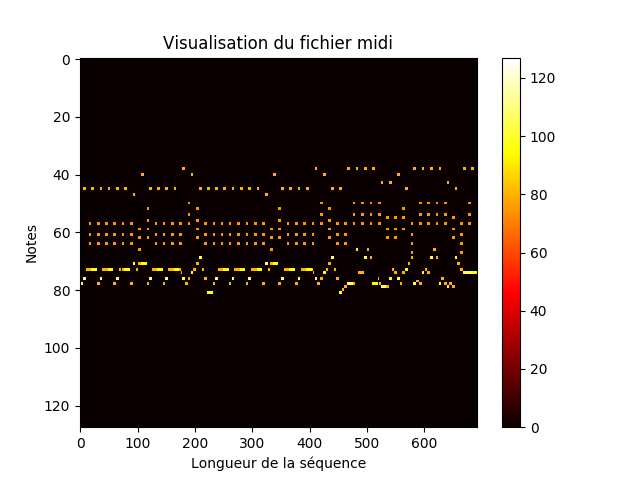
\includegraphics[width=0.5\textwidth]{images/chapter9/jig1.png}\label{jig}}
  \hfill
  \subfloat[Mozart]{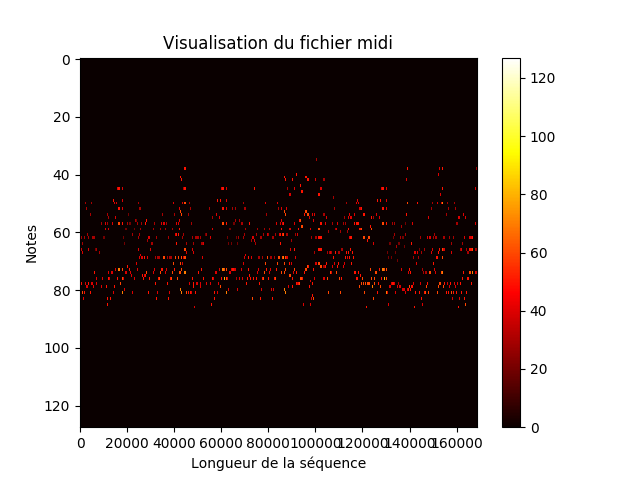
\includegraphics[width=0.5\textwidth]{images/chapter9/mozart.png}\label{mozart}}
  \caption{Visualisation de fichiers midi}
\end{figure}

Lors de l'apprentissage, on envoie en entrée du réseau une colonne de la matrice. Celui-ci doit alors prévoir la prochaine. Lors de la génération, on donne un vecteur ou une séquence de notes en entrée du réseau et on lui demande de générer un morceau de musique. On définit un seuil (à régler, souvent entre 10 et 20) qui permet de décider si une note est active ou non. Cela permet de jouer plusieurs notes en même temps ainsi que des accords. Après la génération d'un vecteur, on ne le remet pas directement en entrée. On sélectionne les notes actives grâce au seuil et on met les autres à 0. On obtient finalement un ensemble de vecteurs décrivant les états successifs du morceau généré. On les concatène pour en faire une matrice. Il ne reste plus qu'à faire la conversion de cette matrice en midi.


\subsection{Résultats}
On applique dans un premier temps l'apprentissage sur les jigs. On utilise deux cellules LSTM en série avec un état caché de 512. On met une couche de neurones pour adapter les données en sortie. Avec une activation linéaire on obtient ainsi des vecteurs de taille 128 en sortie où chaque élément représente l'intensité de la note correspondante. On lui donne en entrée des séquence de 10 vecteurs, cela signifie que l'on va déplier le réseau 10 fois à chaque fois. Un fait des batchs de 50 séquences. On utilise RMSprop comme algorithme d'optimisation avec un learning rate de 0.95. La figure \ref{midi_generated_jigs} permet de visualiser le fichier généré après le passage de 38 800 batchs lors de l'apprentissage.

\begin{figure}[!ht]
  \centering
  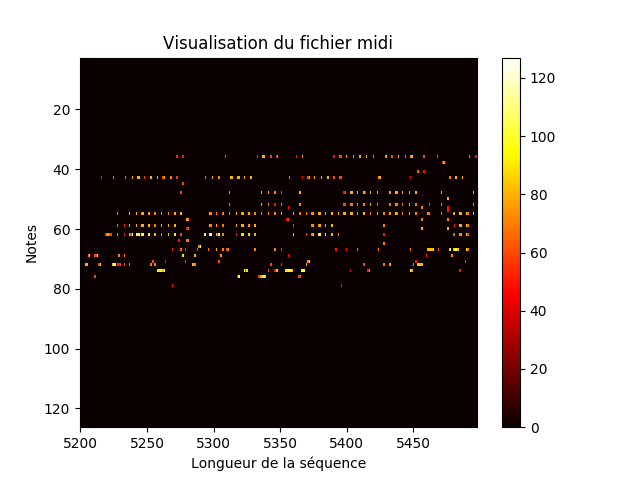
\includegraphics[width=0.5\textwidth]{images/chapter9/midi_generated_jigs_38800.png}
  \caption{Visualisation du fichier midi généré à partir des jigs après 38 800 batchs}
    \label{midi_generated_jigs}
\end{figure}
Le résultat obtenu possède bien le style des jigs avec un accompagnement répétitif à l'arrière. Cet accompagnement, souvent commun aux jigs, est très rapidement appris par le réseau. Certaines séquences mélodiques rappellent énormément certaines jigs de l'apprentissage.

\vspace{2cm}

L'apprentissage de Mozart se fait sur plusieurs symphonies pour piano trouvées dans une base de données de midi. On utilise une fois de plus 2 cellules LSTM en série avec un état caché de 512. Cette fois on fait l'apprentissage sur des séquences de longueur 120. Une longueur plus grande est importante car les morceaux de Mozart sont moins répétitifs que les jigs. Cela permet au réseau de remonter plus loin dans les vecteurs passés et donc d'apprendre la structure de séquences plus longues. On passe des batchs comportant 10 séquences. On utilise là aussi l'algorithme RMSprop avec un learning rate de 0.95. \\
La difficulté principale lors de l'apprentissage de Mozart est que la structure commune des morceaux est moins évidente que dans les jigs. De plus, il y a souvent des changements de rythmes/tempo dans les fichiers midi, ce qui est difficile à retranscrire dans la représentation matricielle avec l'implémentation actuelle. La figure \ref{midi_generated_mozart} représente le morceau généré après 79 500 passés.

\begin{figure}[!h]
  \centering
  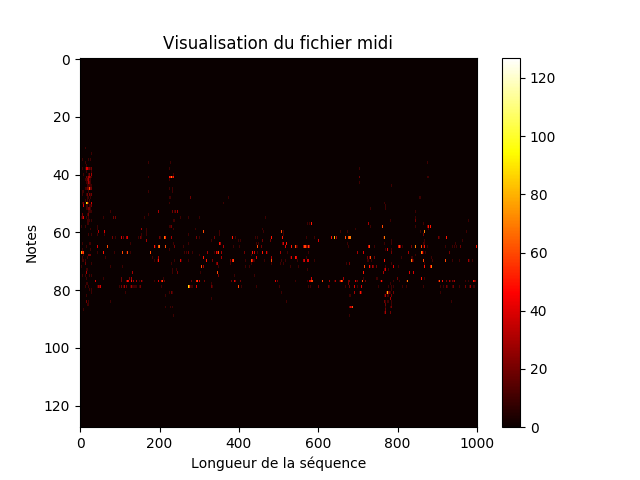
\includegraphics[width=0.5\textwidth]{images/chapter9/midi_generated_mozart_79500.png}
  \caption{Visualisation du fichier midi généré à partir des morceaux de Mozart après 79 500 batchs}
  \label{midi_generated_mozart}
\end{figure}

Il est nécessaire de passer un grand nombre de batchs avant d'avoir des résultats satisfaisants. Le morceau généré a une forme similaire aux morceaux du datasets. Néanmoins, l'écoute ne rend pas toujours aussi bien que les originaux. Un réseau plus complexe, un apprentissage plus long et une base de données plus importante pourraient permettre d'améliorer les résultats.


\section{Génération de partitions}


\section{Génération de signaux}